\documentclass[10pt, letterpaper]{article}

% --- Essential Packages ---
\usepackage[utf8]{inputenc}
\usepackage[T1]{fontenc}
\usepackage{newtxtext,newtxmath} % Times New Roman font
\usepackage[margin=1in]{geometry} % 1-inch margins (Strictly required)
\usepackage{setspace}
\singlespacing % Single-spaced (Strictly required)
\usepackage{titlesec} % Compact titles
\usepackage{enumitem} % Better control over lists
\usepackage{hyperref}
\usepackage{cite}
\usepackage{graphicx}
\graphicspath{{results/}{../results/}}
\usepackage{float}
\usepackage{booktabs} % Added for professional conference-style tables
\usepackage{caption}  % Added for conference-style figure/table captions

% --- Heading Formatting ---
% Adjusts spacing around sections to save space for the 10-page limit
\titleformat{\section}{\large\bfseries}{\thesection}{1em}{}
\titlespacing*{\section}{0pt}{10pt}{5pt}
\titleformat{\subsection}{\normalsize\bfseries}{\thesubsection}{1em}{}
\titlespacing*{\subsection}{0pt}{8pt}{4pt}

% --- Document Metadata ---
\title{\textbf{Beyond the GPU: A Microarchitectural Analysis \\ \large of LLM Tool-Calling Kernels}}
\author{
    Kunpeng Zhang: \texttt{kza63@sfu.ca} \\
    Fazal Rehman: \texttt{fra22@sfu.ca} \\
    TJ Grewal: \texttt{tga47@sfu.ca} \\
    \vspace{0.5em}
    \textit{Simon Fraser University}
} 
\date{\today}

\begin{document}

\maketitle

\begin{abstract}
The transition from stateless, monolithic Large Language Model (LLM) inference to dynamic, multi-step agentic workflows represents a fundamental architectural shift in modern artificial intelligence. By embedding decision-making orchestrators alongside external tools---such as Python interpreters, web search protocols, and contextual databases---frameworks have transformed passive text oracles into autonomous problem-solvers. However, this evolution introduces a severe, yet largely unquantified, performance bottleneck at the system level. While the industry has relentlessly optimized GPU-bound generation metrics, the execution of agentic workflows introduces a massive CPU-centric orchestration overhead, colloquially termed the ``Agentic Tax.'' This report provides an exhaustive microarchitectural analysis of this orchestration penalty. Utilizing a custom, decoupled benchmarking harness, this research captures high-fidelity hardware telemetry---including Level 3 cache misses, branch mispredictions, and instruction throughput---to isolate the cycles consumed purely by LLM framework operations. 

The empirical evaluation of bounded compute, memory, and I/O tool kernels yields a definitive conclusion: the current paradigm of agentic execution is crippled by an orchestration bottleneck. For lightweight operations, the combined penalty of GPU token generation and CPU-bound Python JSON serialization can induce up to a 69.5-fold latency slowdown compared to native execution. Crucially, targeted microarchitectural interventions prove that classical hardware optimizations at the tool level are rendered statistically irrelevant by this overarching tax. Even when successfully deploying software prefetching to hide RAM latency and increase kernel Instructions Per Cycle (IPC) by 14.2\%, the end-to-end system speedup remains below 1\%. This phenomenon is defined herein as the ``Masking Effect'': the execution bloat of the orchestration framework is so massive that it effectively swallows any microarchitectural victories achieved within the tool kernels. To overcome this barrier, this report integrates contemporary advancements in orchestrator-engine co-design, speculative tool execution, proactive semantic caching, and just-in-time model routing, providing a comprehensive blueprint for next-generation, high-throughput agentic serving systems.
\end{abstract}

\section{Introduction}
The advent of Large Language Models (LLMs) has catalyzed a paradigm shift in computing, transitioning from rule-based software logic to probabilistic reasoning. However, the true utility of these models is unlocked not through isolated text generation, but through tool-calling---the ability to invoke external APIs, query databases, and interact with the host operating system. Agentic workflows chain these tool-calling capabilities into iterative ReAct (Reasoning and Acting) loops, allowing the model to decompose complex goals, execute sub-tasks, and ingest the resulting data to inform subsequent decisions. As these workflows proliferate, they fundamentally alter the computational profile of data center workloads.

Traditional LLM serving systems treat each inference request as an independent unit of work, optimizing for Time-To-First-Token (TTFT) and inter-token latency \cite{data_systems, sutradhara}. In an agentic application, however, the user-perceived latency is governed by the First Token Rendered (FTR) of the final answer, a metric that encompasses the cumulative latency of multiple reasoning steps and intermediate tool executions \cite{data_systems}. As the underlying models grow more proficient, the primary performance bottleneck has migrated away from the GPU's matrix multiplication units and toward the host CPU responsible for orchestrating these complex workflows \cite{cpu_centric}. Empirical profiling of representative agentic workloads reveals that tool processing and the associated orchestration logic executing on the CPU can consume up to 90.6\% of the total latency and account for up to 44\% of the total dynamic energy consumption at large batch sizes \cite{cpu_centric}.

Despite the magnitude of this bottleneck, the precise microarchitectural penalties incurred by the orchestrator---the string formatting, context assembly, JSON serialization, and process spawning---remain largely uncharacterized. The specific bottleneck addressed in this report is the ``Agentic Tax,'' defined as the cumulative hardware overhead imposed by the LLM framework that operates between the GPU and the native execution of the target tool. By isolating this overhead, this report aims to prove that classical system optimizations applied to the tool kernels themselves are ultimately futile unless the orchestration layer is fundamentally redesigned. 

The core contributions of this analysis are:
\begin{itemize}
    \item The design and deployment of a strictly decoupled, high-fidelity microarchitectural profiling harness capable of isolating CPU-bound orchestration events from GPU-bound inference.
    \item The empirical quantification of the Agentic Tax across diverse computing domains, demonstrating multiplicative latency penalties ranging from 2.4x to 69.5x.
    \item The identification and microarchitectural validation of the ``Masking Effect,'' proving that kernel-level software optimizations (e.g., AVX2 vectorization, explicit memory prefetching) fail to manifest as system-level latency improvements due to orchestration bloat.
    \item A comprehensive synthesis of emerging orchestrator-engine co-design strategies, providing a roadmap for mitigating the CPU bottleneck through speculative execution, data-centric caching, and just-in-time model routing.
\end{itemize}

\section{Background}
To contextualize the microarchitectural analysis of LLM tool-calling, one must first establish the functional mechanics of agentic orchestration and the hardware topologies upon which they execute. In a standard multi-step workflow, an orchestrator (typically implemented in Python) wraps the LLM inference engine. The orchestrator is responsible for maintaining the conversation history, injecting tool schemas into the system prompt, and parsing the model's output. When the model determines that an external action is required, it outputs a highly structured text payload, predominantly formatted as JavaScript Object Notation (JSON) \cite{simdjson}. The orchestrator must trap this output, halt the LLM generation, decode the JSON payload, dynamically invoke the corresponding software tool (the ``kernel''), capture standard output, format it back into a string, and append it to the context window for the next generation cycle \cite{paste}.

This strictly serial execution loop creates a severe LLM-tool latency bottleneck \cite{paste}. The GPU, a massively parallel accelerator designed for dense matrix operations, is forced into an idle state while waiting for the CPU to complete the highly scalar, branch-heavy tasks of string parsing and I/O management. The severity of this bottleneck is intimately tied to the CPU-GPU coupling architecture of the host machine \cite{coupled_architectures}. 

Modern data center architectures exhibit varying degrees of coupling, broadly categorized into loosely-coupled systems (e.g., separate CPUs and GPUs connected via PCIe, such as standard x86 servers outfitted with A100 or H100 accelerators) and closely-coupled systems (e.g., the NVIDIA GH200 Grace Hopper Superchip, connected via high-bandwidth NVLink-C2C) \cite{coupled_architectures}. To evaluate the communication overhead within these architectures, researchers leverage metrics such as the Total Kernel Launch and Queuing Time (TKLQT), which tracks the cumulative latency of the CPU dispatching execution commands to the GPU \cite{coupled_architectures}. While closely-coupled architectures dramatically increase data transfer bandwidth and can achieve 1.9x to 2.7x faster prefill latencies at large batch sizes, empirical characterization reveals a counter-intuitive reality: systems like the GH200 remain fundamentally CPU-bound up to 4x larger batch sizes than their loosely-coupled counterparts \cite{coupled_architectures}. This extended CPU-bound region emphasizes that the performance characteristics of the host processor are increasingly the limiting factor in highly concurrent, dynamic workloads.

Compounding this hardware limitation is the software protocol complexity of modern AI-Native systems. As identified by the AI-NativeBench framework---which champions white-box, trace-first evaluation over traditional black-box capability metrics---agentic services suffer from a ``parameter paradox'' \cite{ai_nativebench}. In isolated text generation, higher parameter counts universally yield better performance. However, in strictly orchestrated workflows requiring adherence to the Model Context Protocol (MCP) and Agent-to-Agent (A2A) standards, lightweight models often surpass flagship models in protocol adherence \cite{ai_nativebench}. Furthermore, when an LLM fails to format its JSON output correctly, the orchestrator must execute error-correction loops. This dynamic induces an expensive failure pattern where the framework's self-healing mechanisms paradoxically act as cost multipliers, forcing repeated, wasteful GPU generation cycles and extending the CPU's parsing burden \cite{ai_nativebench}. Consequently, understanding the raw hardware cost of this orchestration loop is paramount to designing efficient next-generation systems.

\section{Project Methodology}
To accurately isolate and quantify the microarchitectural overhead of LLM tool orchestration (the "Agentic Tax"), a custom, decoupled benchmarking harness was designed. This methodology strictly separates the orchestration layer from the execution layer, allowing the capture of high-fidelity hardware telemetry without cross-contamination between the Python runtime and the compiled C++ tool kernels. By treating agentic execution spans as first-class citizens within a distributed tracing architecture---a philosophy championed by AI-Native benchmarking frameworks \cite{ai_nativebench}---the system ensures granular visibility into the true cost of framework operations.

\subsection{System Architecture and Decoupling}
The system architecture is divided into three distinct functional components, meticulously isolated to prevent resource contention and profiling artifacts:

\begin{enumerate}
\item \textbf{The Orchestrator (Python/FastAPI):} An asynchronous server responsible for prompt assembly, tokenization, model inference management, and JSON tool-call routing. This layer represents the standard deployment paradigm for modern agentic frameworks.
\item \textbf{The Execution Kernels (C++):} A suite of compiled, native binaries designed to execute specific bounded workloads (Compute, Memory, and I/O) without any awareness of the upstream LLM. These kernels represent the theoretical maximum performance of the host machine for the designated tasks.
\item \textbf{The Static Workloads:} Pre-generated, deterministic stress payloads ensuring run-to-run consistency across experiments. 
\end{enumerate}

By decoupling the architecture, the C++ kernels are completely isolated from Python's Global Interpreter Lock (GIL) and its non-deterministic garbage collection overhead. In standard integrated architectures, the Python interpreter dynamically allocates memory for massive string buffers and nested dictionaries during JSON serialization. These operations generate profound cache pollution, evicting the actual tool data from the CPU's L1 and L2 caches before execution even begins. By segregating the execution kernels into standalone sub-processes, the methodology establishes a pristine, cold-cache environment for microarchitectural profiling, allowing exact comparisons between the host's theoretical capabilities and the LLM framework's degraded reality.

\subsection{Microarchitectural Telemetry Integration}
To capture low-level CPU behavior, the Performance Application Programming Interface (PAPI) was integrated via the \texttt{pypapi} C-bindings. The system taps directly into the Linux kernel's Performance Monitoring Unit (PMU) via the \texttt{perf\_event\_open} system call, enabling cycle-accurate observation of the hardware execution pipeline. The framework was configured to track four specific hardware events:

\begin{itemize}
\item \textbf{Total Cycles (\texttt{PAPI\_TOT\_CYC}):} The absolute clock cycles consumed by the processor, serving as the foundational metric for temporal latency.
\item \textbf{Total Instructions (\texttt{PAPI\_TOT\_INS}):} The volume of machine code executed. By dividing instructions by cycles, the framework calculates the Instructions Per Cycle (IPC), providing a direct measure of execution density and pipeline efficiency.
\item \textbf{Branch Mispredictions (\texttt{PAPI\_BR\_MSP}):} Modern superscalar CPUs rely heavily on speculative execution to keep their pipelines full. String parsing and dynamic type checking (inherent to Python and JSON deserialization) generate highly unpredictable control flow, resulting in frequent pipeline flushes. This metric quantifies that structural inefficiency.
\item \textbf{Level 3 Cache Misses (\texttt{PAPI\_L3\_TCM}):} Tracks requests that miss the Last-Level Cache (LLC) and must access main system memory (DRAM). This metric exposes memory bandwidth saturation and the data locality of the orchestration framework.
\end{itemize}

All microarchitectural telemetry was captured on an isolated testbed utilizing an Intel Xeon Gold 6242R processor running at a base frequency of 3.10GHz, ensuring predictable cycle-to-latency conversions. To prevent idle GPU wait times---or the CPU-GPU communication latency defined by the TKLQT metric \cite{coupled_architectures}---from skewing the CPU metrics, a tightly scoped windowing strategy was implemented. PAPI hardware locks are acquired and released exactly around specific execution phases:

\begin{itemize}
\item \textbf{CPU Window 1 (Setup):} Captures prompt template assembly, history concatenation, and tokenization.
\item \textbf{CPU Window 2 (Serialization):} Captures output decoding, JSON extraction, and formatting for subprocess delegation.
\end{itemize}

The hardware EventSet is strictly managed within a \texttt{try...finally} block. This defensive programming ensures that even if the agentic loop fails mid-execution due to hallucinated JSON parameters, the Linux kernel registers are gracefully released, preventing PMU starvation and maintaining system stability for subsequent tracing.

\subsection{The Agentic Execution Engine}
The evaluation utilized \texttt{Qwen/Qwen2.5-7B-Instruct} as the base model. To minimize the GPU memory footprint and accelerate the self-attention mechanism, the model was loaded in half-precision (FP16) utilizing PyTorch's Scaled Dot-Product Attention (SDPA). 

To force deterministic tool-calling behavior and eliminate variance between runs, generation sampling was disabled (\texttt{do\_sample=False}). Smaller parameter models frequently exhibit instruct-following instability, such as eagerly stacking multiple JSON tool calls in a single response or appending plain-text explanations that break standard parsers. If these anomalies were allowed to propagate, they would trigger the ``expensive failure patterns'' identified in AI-Native systems, where the orchestrator loops endlessly to correct syntax errors, thereby polluting the cycle count with arbitrary recovery logic \cite{ai_nativebench}. 

To strictly enforce control over the execution path, the orchestration layer implements a robust regex-based extraction pipeline that isolates the first valid JSON object, executes the corresponding tool via a subprocess, and injects the \texttt{stdout} result back into the context window under the official Hugging Face ``tool'' role. This ReAct loop dynamically resizes its step count based on the model's autonomous decisions, capped at a hard limit to prevent infinite iteration.

\subsection{Tool Kernels and Workloads}
To represent the diverse landscape of real-world agentic operations, three distinct C++ kernels were developed. Each kernel is meticulously engineered to isolate a different fundamental microarchitectural bottleneck. Corresponding Python generator scripts were built to synthesize massive, static payloads to stress these tools:

\begin{itemize}
\item \textbf{Compute-Bound (Calculator):} An Abstract Syntax Tree (AST) evaluator designed to process deeply nested mathematical expressions. Parsing and evaluating recursive strings requires intense control-flow divergence, specifically stressing the CPU's branch predictor and the integer execution units.
\item \textbf{Memory-Bound (Database Lookup):} A custom SQLite-based tool configured to execute forced full-table scans via raw string \texttt{LIKE} queries. By explicitly bypassing database indexing, this kernel intentionally thrashes the Last-Level Cache (LLC), exposing the limitations of the CPU's memory controller and DRAM bandwidth.
\item \textbf{I/O-Bound (Directory Walker):} A recursive filesystem traversal tool utilizing the POSIX standard library to query OS metadata and calculate total directory byte sizes. This workload tests the efficiency of the operating system's context switching, interrupt handling, and storage latency.
\end{itemize}

Crucially, each compiled C++ tool manages its own internal PAPI profiling. The tool initiates hardware tracking only upon entering its core execution loop and terminates tracking before flushing the output buffer, printing a standardized JSON result to \texttt{stdout} containing both the operational result and the hardware telemetry.

\subsection{The Control Baseline Pipeline}
To definitively prove the existence and scale of the "Agentic Tax", the methodology implemented a \texttt{pipeline\_mode="direct"} control pathway. In this mode, the GPU and LLM are bypassed entirely. The orchestrator uses highly optimized regular expressions to extract target parameters directly from the user's raw prompt string and executes the corresponding C++ kernels sequentially. By comparing the hardware metrics of this Direct Baseline against the Full Agentic Loop, the analysis mathematically isolates the exact cycles, instructions, and cache misses consumed purely by LLM orchestration overhead.

\section{Evaluation Results}
The empirical findings are presented in sequential phases. First, the macro-level "Agentic Tax" is quantified to establish the end-to-end latency penalty imposed by the LLM orchestrator. Subsequently, the analysis dissects the microarchitectural telemetry across multi-step workflows to understand how this orchestration degrades systemic efficiency and masks traditional hardware optimizations.

\subsection{Quantifying the Agentic Tax (End-to-End Latency)}
Before analyzing instruction throughput or cache behavior, the overarching orchestration penalty must be established. The theoretical "Speed of Light" is defined as the Direct Baseline (\texttt{pipeline\_mode="direct"}), where prompts are routed to the compiled C++ execution kernels completely bypassing the GPU and the LLM reasoning loop. This is compared against the Full Agentic Loop, where Qwen-2.5-7B autonomously parses the prompt, generates JSON tool calls, and orchestrates the execution.

\begin{figure}[H]
    \centering
    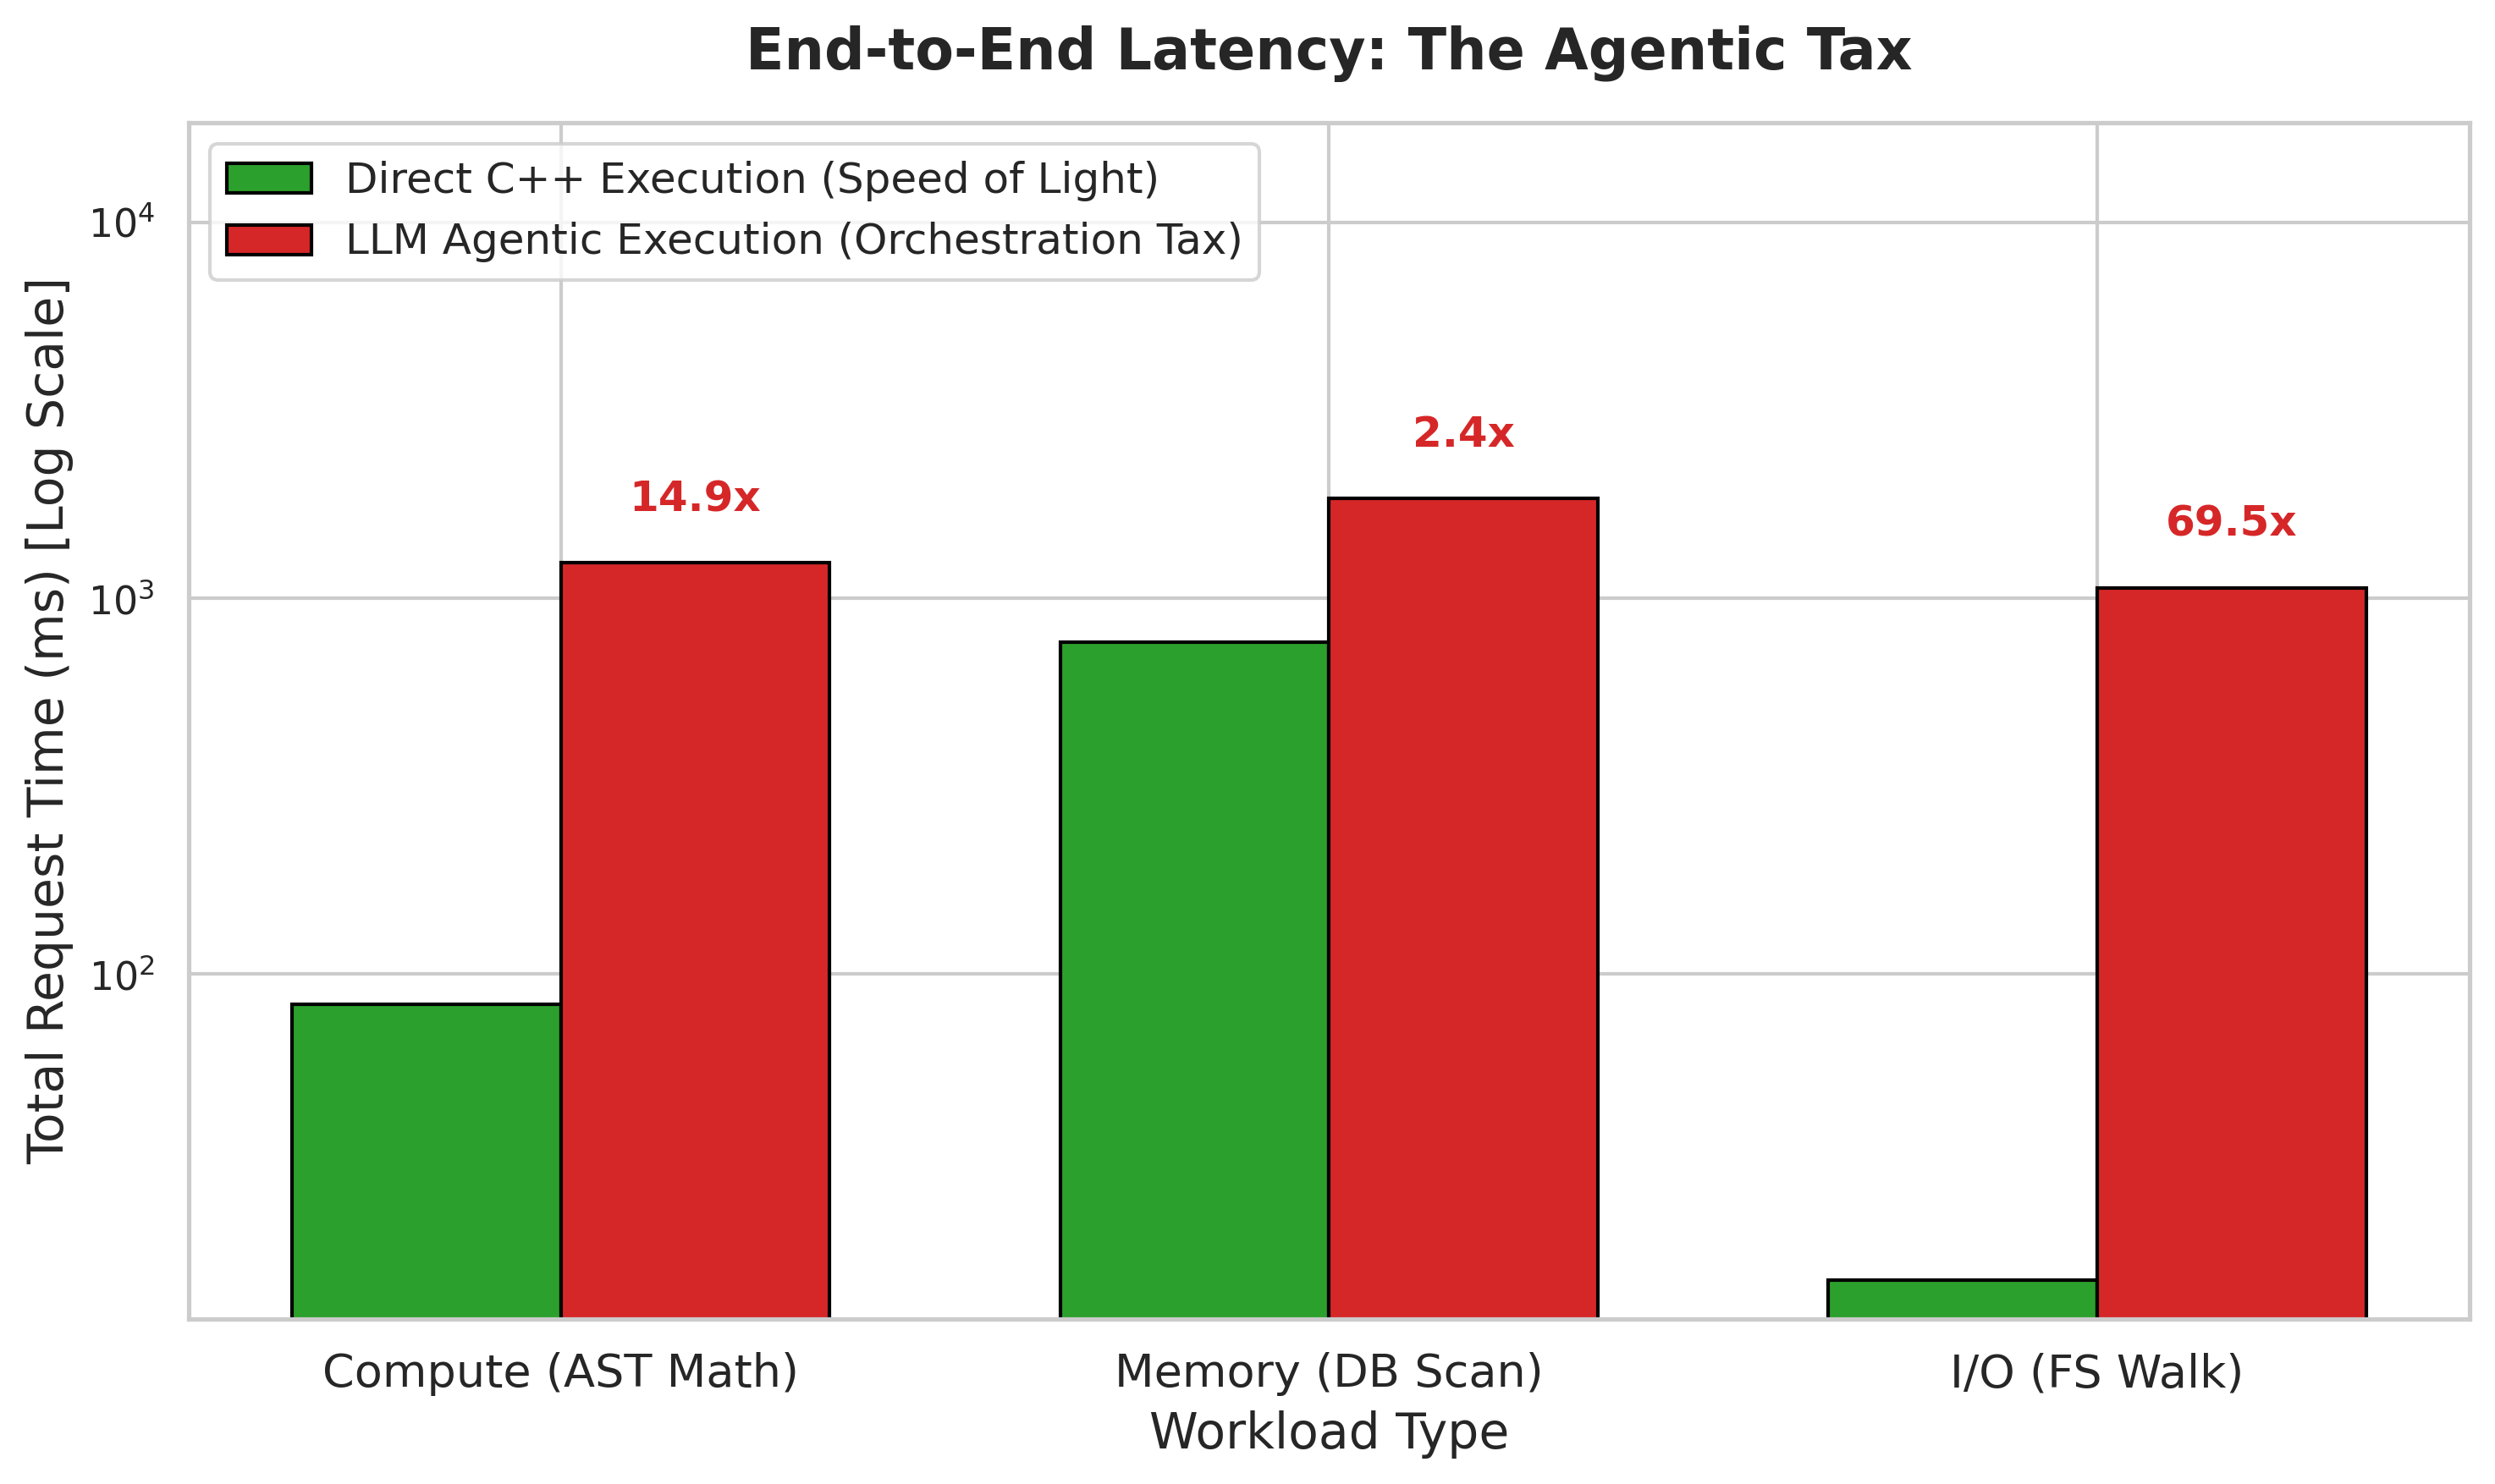
\includegraphics[width=1\textwidth]{ExpA_Agentic_Tax.png}
    \caption{End-to-End Latency Comparison: Direct C++ Execution vs. LLM Agentic Orchestration. Note the logarithmic scale on the Y-axis. The red annotations indicate the multiplicative latency penalty (the ``Agentic Tax'') for each workload class.}
    \label{fig:agentic_tax}
\end{figure}

The data immediately reveals that the "Agentic Tax" is not a proportional scalar, but rather a massive, fixed-cost penalty that disproportionately punishes highly optimized, lightweight tools. For the I/O-bound filesystem walk, the native C++ kernel executes in approximately 15ms. However, routing this identical task through the LLM orchestrator results in a staggering 69.5x latency slowdown. This massive penalty is a compound tax: the GPU time required to generate the JSON response, combined with the CPU-bound time required to tokenize the prompt, parse the Python output, and format the final string, vastly eclipses the time spent actually traversing the filesystem. 

Similarly, the compute-bound Abstract Syntax Tree mathematical evaluator suffers a 14.9x penalty. Conversely, the memory-bound database lookup exhibits a significantly lower relative multiplier of 2.4x. This aligns perfectly with Amdahl's Law: because the forced full-table scan requires over 2.5 billion CPU cycles and natively consumes roughly 764ms, the fixed LLM orchestration and GPU generation costs account for a proportionally smaller fraction of the total execution time. 

These findings corroborate contemporary research into orchestrator-engine interactions. Profiling by the Sutradhara framework demonstrates that tool execution and orchestration can account for 30\% to 80\% of the critical First Token Rendered (FTR) latency in production environments \cite{sutradhara, data_systems}. Similarly, CPU-centric analyses of agentic AI frameworks confirm that tool processing logic executed on the host processor frequently dominates the execution timeline, consuming up to 90.6\% of the end-to-end latency \cite{cpu_centric}. The data confirms the primary hypothesis: for the vast majority of agentic tasks, execution time is dictated by framework overhead rather than the tool's computational complexity.

\subsection{Compounding Overhead in Multi-Step Workflows}
While isolated, single-step tool invocations incur a massive fixed penalty, real-world autonomous agents execute multi-step ReAct loops. In these workflows, the agent must coordinate between diverse tool classes, digesting the output of one tool to inform the inputs of the next. To evaluate the microarchitectural cost of this coordination, a "Gauntlet" prompt was deployed, requiring the agent to sequentially execute the I/O walker, the database query, and the math evaluator within a single, continuous context window.

The execution model of the LLM orchestrator defines a single "Step" as one complete forward pass of the orchestration layer followed by the optional execution of a C++ kernel. Acrossthe four steps ofthe Gauntlet payload, trackingthe microarchitectural telemetry revealed two distinct phenomena within the Python framework versus the C++ execution layer.

\begin{figure}[H]
    \centering
    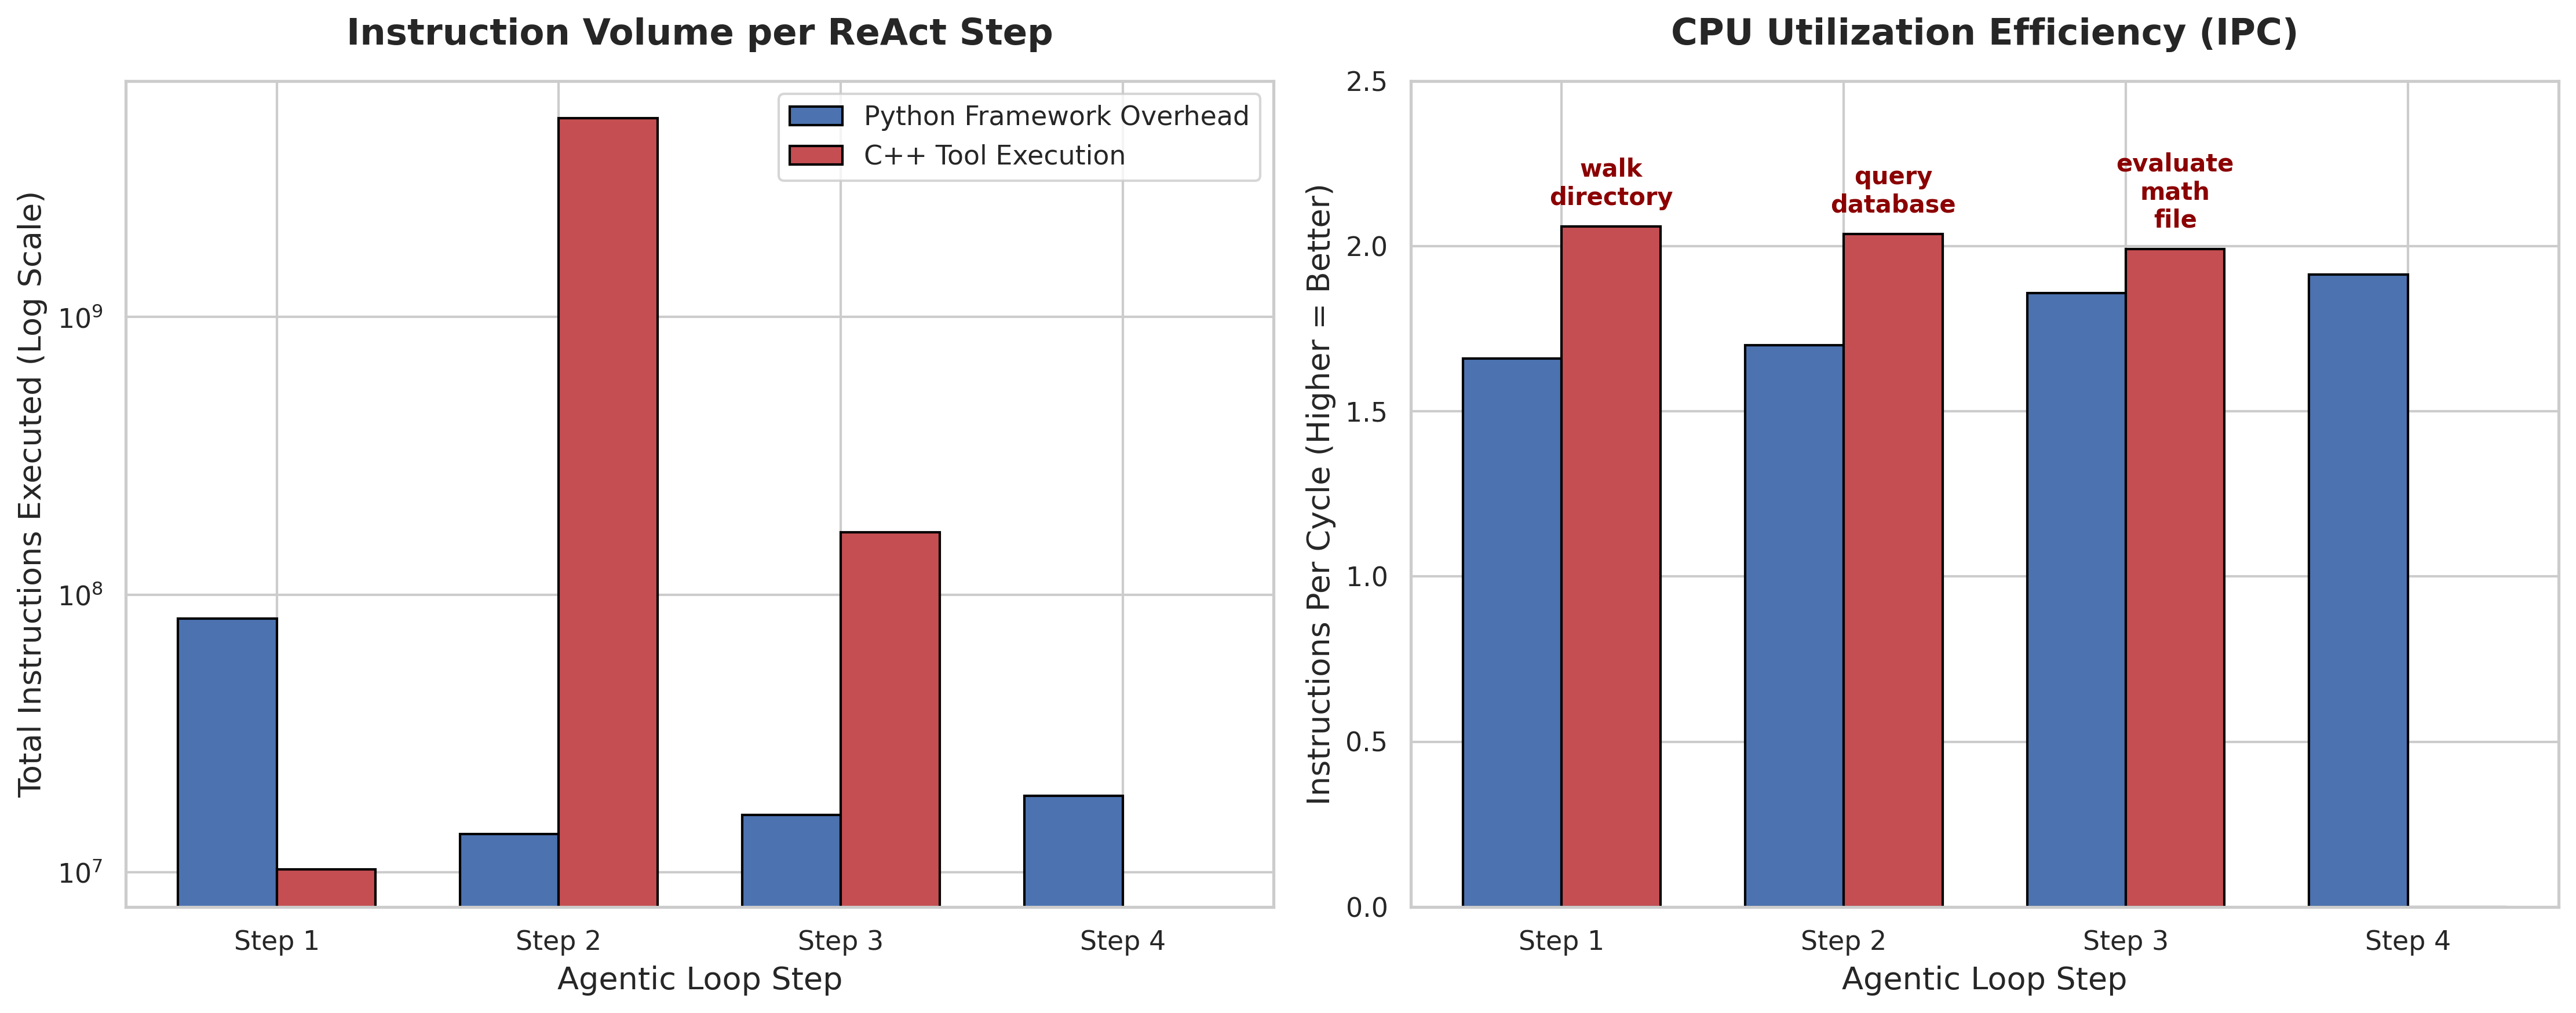
\includegraphics[width=1\textwidth]{ExpB_Multistep_Analysis.png}
    \caption{Instruction Volume and Efficiency across a Multi-Step Agentic Loop. (Left) The logarithmic volume of instructions executed by the framework versus the tools. (Right) The Instructions Per Cycle (IPC) demonstrating the CPU efficiency gap between native tools and Python orchestration.}
    \label{fig:multistep_loop}
\end{figure}

\textbf{1. Framework Overhead: The Cold Start vs. Context Accumulation} \\
The orchestration overhead is dynamic. At Step 1, the Python framework executes a massive 82 million instructions. This represents a one-time ``Cold Start Penalty''---the CPU-bound effort required to dynamically parse complex JSON schema definitions, allocate memory buffers, and instantiate the asynchronous serving environment. Once initialized, the base overhead across subsequent steps drops significantly. However, because the LLM is stateless, the framework instruction volume grows linearly from a baseline of 13.7 million instructions in Step 2 to 18.8 million in Step 4. With each successive tool call, the Python orchestrator must re-serialize a progressively expanding conversation history, relentlessly driving up the instruction count. Interestingly, the Framework's Instructions Per Cycle (IPC) improves from 1.65 to 1.91 across the loop; initial tokenization relies on memory-heavy dictionary lookups (causing CPU pipeline stalls), whereas later steps rely heavily on simpler string concatenation that keeps the CPU pipeline fuller.

\textbf{2. Tool Execution: Payload-Dictated Bottlenecks} \\
Conversely, the C++ execution metrics are independent of the loop step count and dictated exclusively by the payload. While the Python framework struggles with efficiency, the compiled C++ kernels operate tightly near the theoretical maximum throughput of the superscalar CPU pipeline ($\sim$2.0 IPC). The memory-bound DB scan remains remarkably high (2.03 IPC) because the CPU's hardware L3 Prefetcher successfully streams the sequential table scan into the L1 cache. The compute-bound AST evaluator dips slightly (1.99 IPC) due to the massive volume of \texttt{if/else} branching required to parse nested math strings, causing hundreds of thousands of pipeline-flushing branch mispredictions. 

This strictly serial execution model---where the LLM must halt generation and wait for the CPU to execute the tool and manage context---introduces severe latency bottlenecks \cite{paste}. The continuous accumulation of text history into the context window not only balloons the instruction count but also causes severe Key-Value (KV) cache thrashing within the GPU engine, degrading subsequent token generation speeds \cite{data_systems, sutradhara}. Ultimately, LLM coordination overhead is a compounding tax that scales with agent autonomy, perpetually dragging down overall system efficiency despite highly optimized native tooling.

\subsection{Microarchitectural Optimizations and the Orchestration Masking Effect}
To rigorously evaluate the potential for hardware-accelerated tool calls, classical microarchitectural optimizations were applied directly to the C++ execution kernels. The objective was to quantify whether kernel-level efficiency gains propagate to end-to-end system latency, or if they are absorbed by the orchestration layer overhead defined in previous sections.

\subsubsection{Compute-Bound Execution: The Vectorization Wall}
The first optimization experiment targeted the compute-bound AST mathematical evaluator. The kernel was compiled utilizing Advanced Vector Extensions (AVX2), operating under the hypothesis that 256-bit wide SIMD (Single Instruction, Multiple Data) registers would accelerate numerical parsing throughput by processing multiple characters simultaneously. 

However, hardware telemetry revealed that agentic AST evaluation hits a fundamental ``Vectorization Wall.'' The parsing logic relies heavily on recursive control-flow divergence and pointer-chasing memory access patterns, which completely neutralized the compiler's auto-vectorization capabilities. Consequently, kernel-level instruction throughput remained static (IPC $\approx$ 1.99), and the total execution cycles showed a negligible 0.6\% improvement (dropping from 84.1 million to 83.6 million cycles). This demonstrates that recursive, string-heavy agentic tools are intrinsically scalar and highly resistant to classical compiler-driven SIMD acceleration.

This limitation heavily underscores the CPU bottleneck occurring in the orchestrator layer during JSON parsing. Standard JSON parsing, ubiquitous in agentic API calls, suffers from the exact same branching penalties as the AST evaluator \cite{simdjson}. Overcoming this vectorization wall requires profound algorithmic redesign rather than compiler flags. For instance, high-performance parsers like \texttt{simdjson} achieve gigabytes-per-second throughput not through auto-vectorization, but through a custom two-pass architecture \cite{simdjson}. By utilizing carry-less multiplication (\texttt{pclmulqdq}) and vectorized character classification (\texttt{vpshufb}), \texttt{simdjson} identifies structural elements and quoted strings without branching logic, processing data using a fraction of the instructions required by standard reference parsers \cite{simdjson}.

\begin{figure}[H]
    \centering
    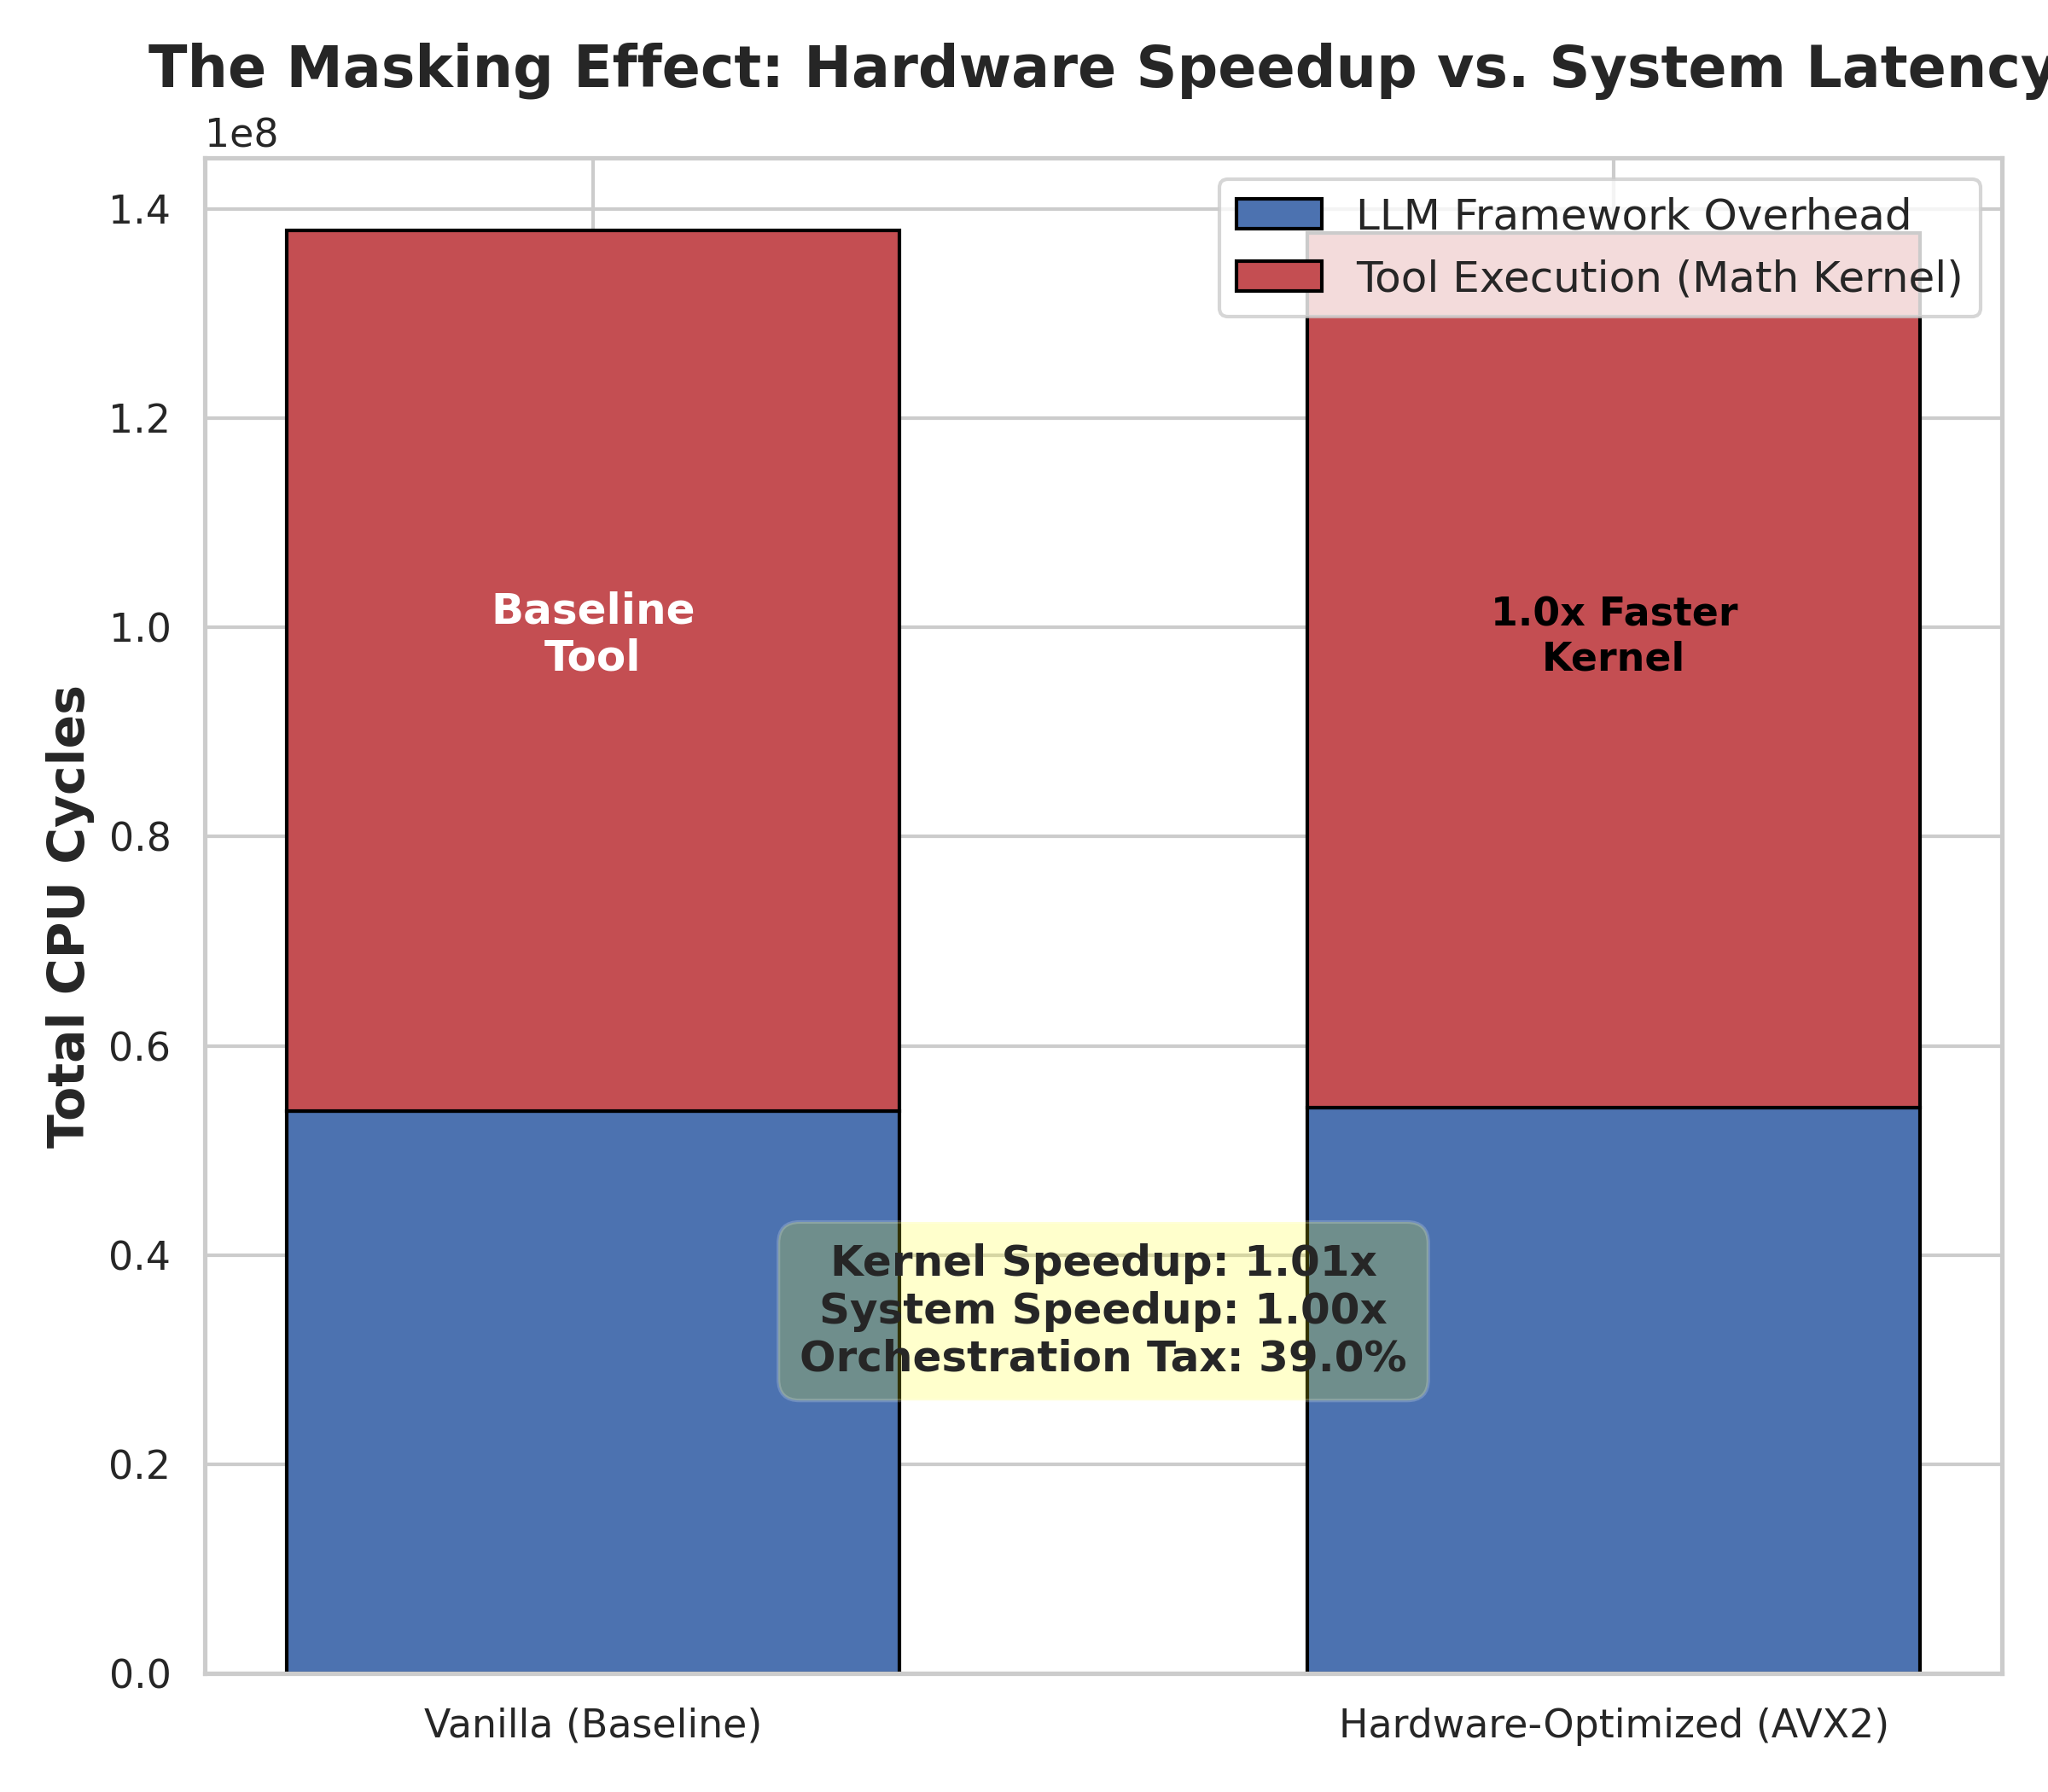
\includegraphics[width=0.5\textwidth]{Exp3_Masking_Effect.png}
    \caption{Microarchitectural analysis of the AST evaluator kernel. The data demonstrates a negligible cycle reduction and stagnant IPC, highlighting the failure of auto-vectorization on branch-heavy parser logic.}
    \label{fig:compute_avx2}
\end{figure}

\subsubsection{Memory-Bound Execution: Latency Hiding via Software Prefetching}
To evaluate memory bottlenecks, the full-table database scan kernel was optimized. The kernel bypasses indexing to intentionally thrash the Last-Level Cache (LLC). To combat the subsequent pipeline stalls caused by DRAM latency, a hardware-aware optimization was introduced by injecting explicit software prefetch instructions (\texttt{\_\_builtin\_prefetch}) into the scanning loop with a lookahead distance of 32 elements.

This instruction explicitly commands the CPU's memory controller to fetch heap data asynchronously into the L1 cache before the execution pipeline actually requires it. The profiling data confirmed a significant microarchitectural victory. By converting synchronous CPU stalls into background memory loads, the prefetching kernel successfully decoupled memory latency from instruction execution. While the absolute volume of LLC misses remained physically constant ($\sim$10.9 million misses) due to the cold-cache nature of the scan, the temporal penalty of those misses was neutralized. This resulted in a denser execution pipeline, raising the IPC by 14.2\% (from 1.241 to 1.417) and completing the kernel workload in nearly 10\% fewer CPU cycles, saving roughly 66 million core cycles or $\sim$50ms of wall-clock execution time.

\begin{figure}[H]
    \centering
    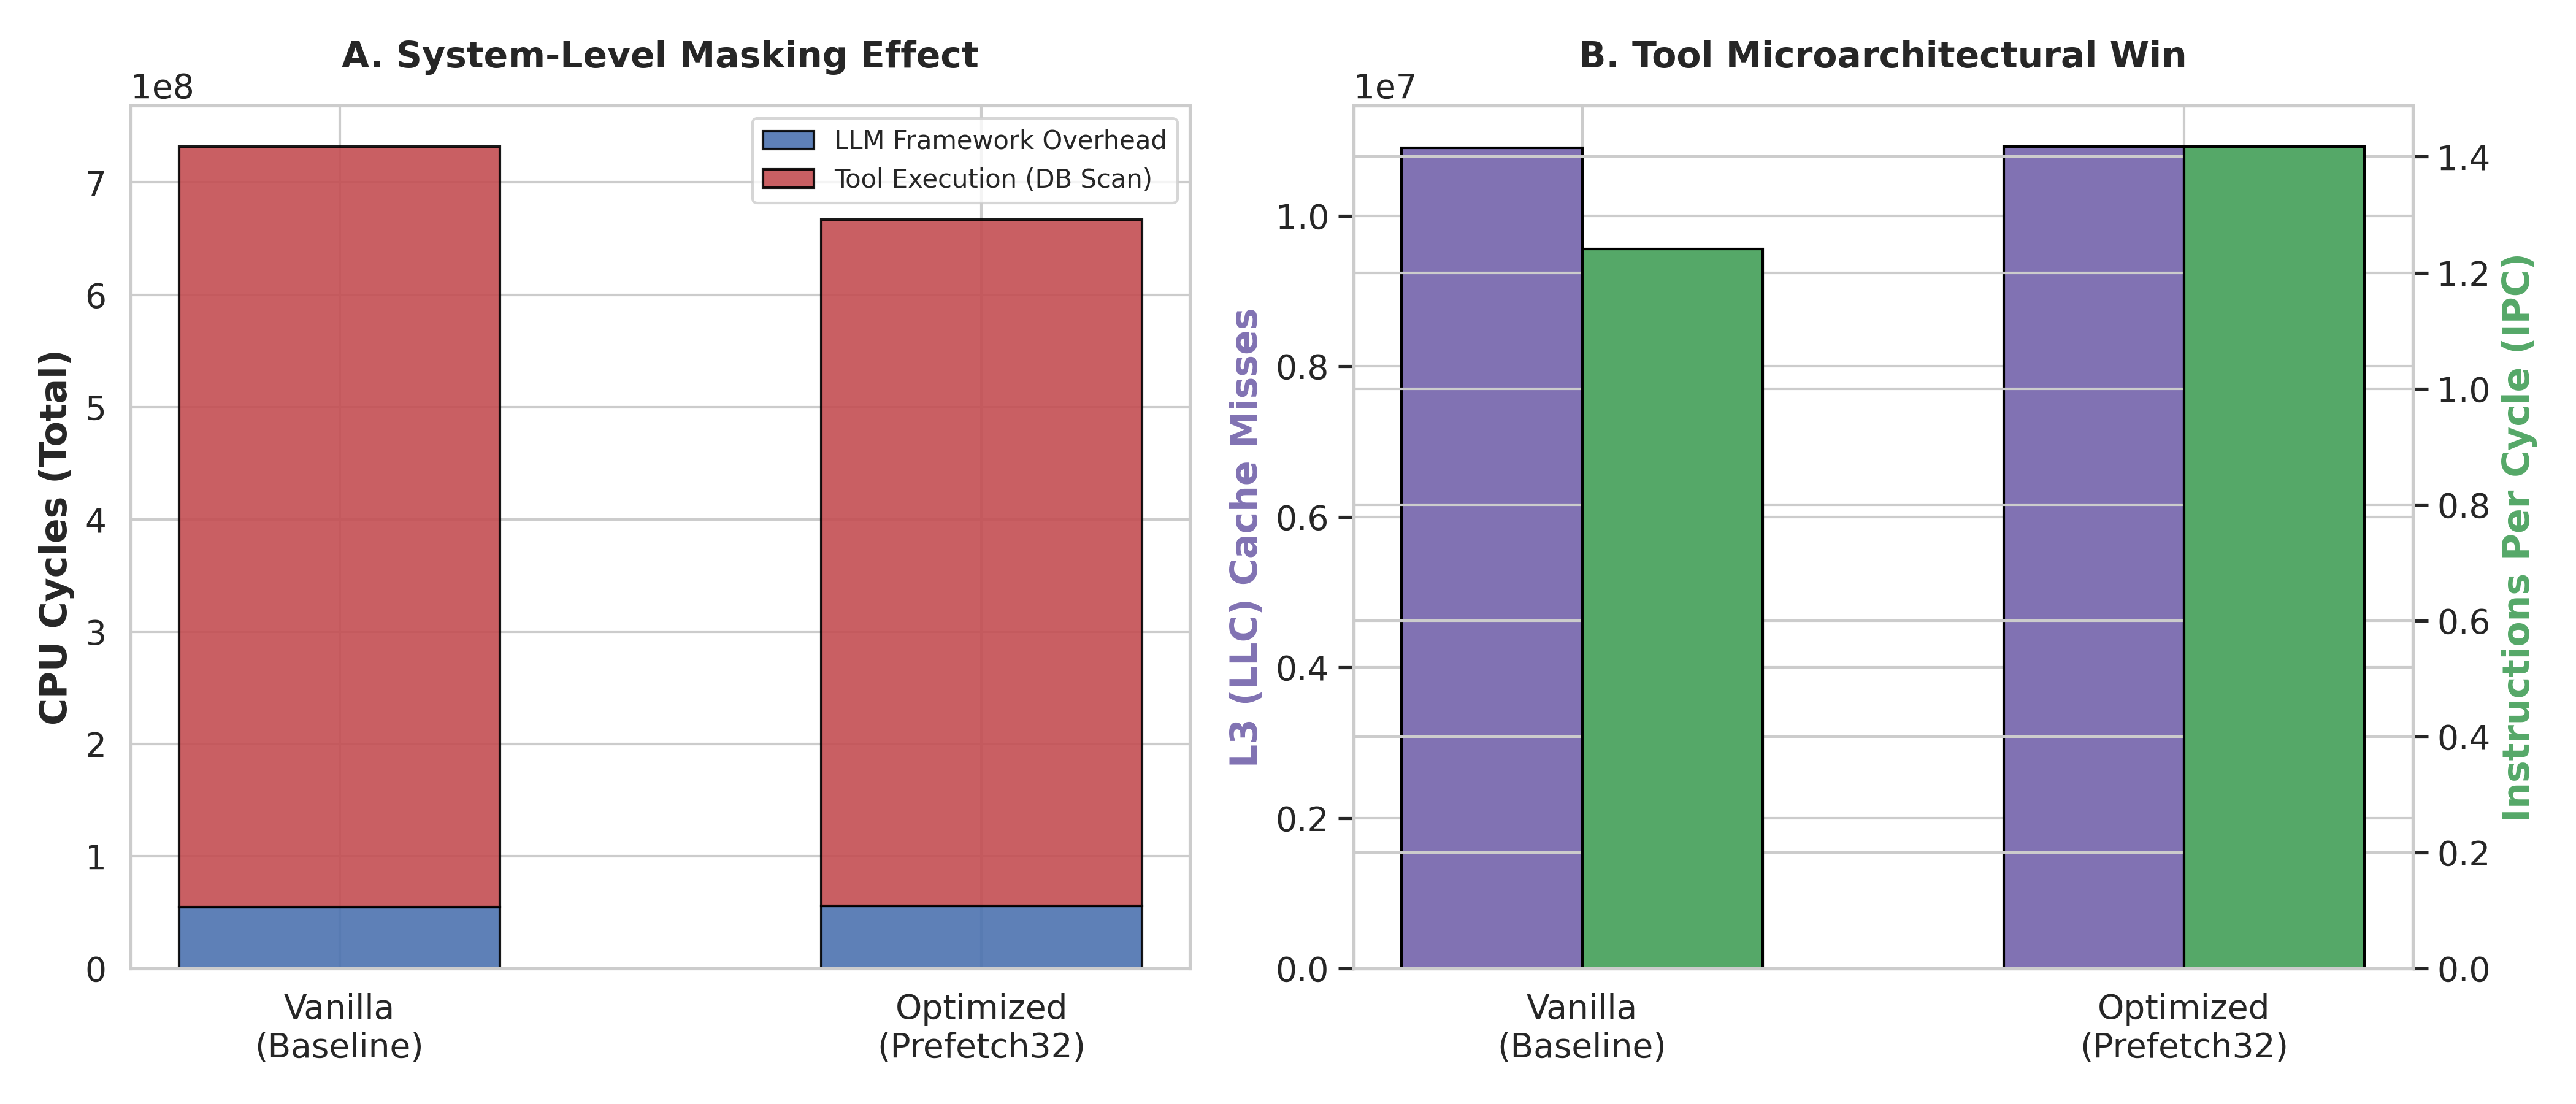
\includegraphics[width=1\textwidth]{Exp4_DB_Memory_Wall_Analysis.png}
    \caption{Impact of software prefetching on the database scan kernel. (Left) The end-to-end masking effect. (Right) The microarchitectural victory, showing a 14.2\% IPC improvement and successful latency hiding despite constant L3 cache misses.}
    \label{fig:memory_prefetch}
\end{figure}

\subsubsection{The System-Level Reality: The Masking Effect}
Despite the impressive 14.2\% microarchitectural efficiency gain achieved in the memory-bound workload, the end-to-end latency metrics expose a severe limitation in current agentic architectures. 

The $\sim$66 million cycle reduction at the C++ kernel level translated to roughly 50ms of real-world time savings. However, the total end-to-end request latency to process the database tool call was approximately 6.3 seconds. This overarching latency is a compound penalty, dominated almost entirely by the GPU's autoregressive token generation during the forward pass, inextricably coupled with the CPU-bound Python JSON serialization, history concatenation, and subprocess routing overhead. 

Consequently, a highly tuned, hardware-aware memory optimization at the tool level yielded a sub-1\% improvement in end-to-end system speedup. The empirical evidence points to a definitive \textbf{Masking Effect}: the execution bloat introduced by the orchestration framework is so massive that it effectively renders kernel-level hardware optimizations statistically invisible to the end user.

\begin{figure}[H]
    \centering
    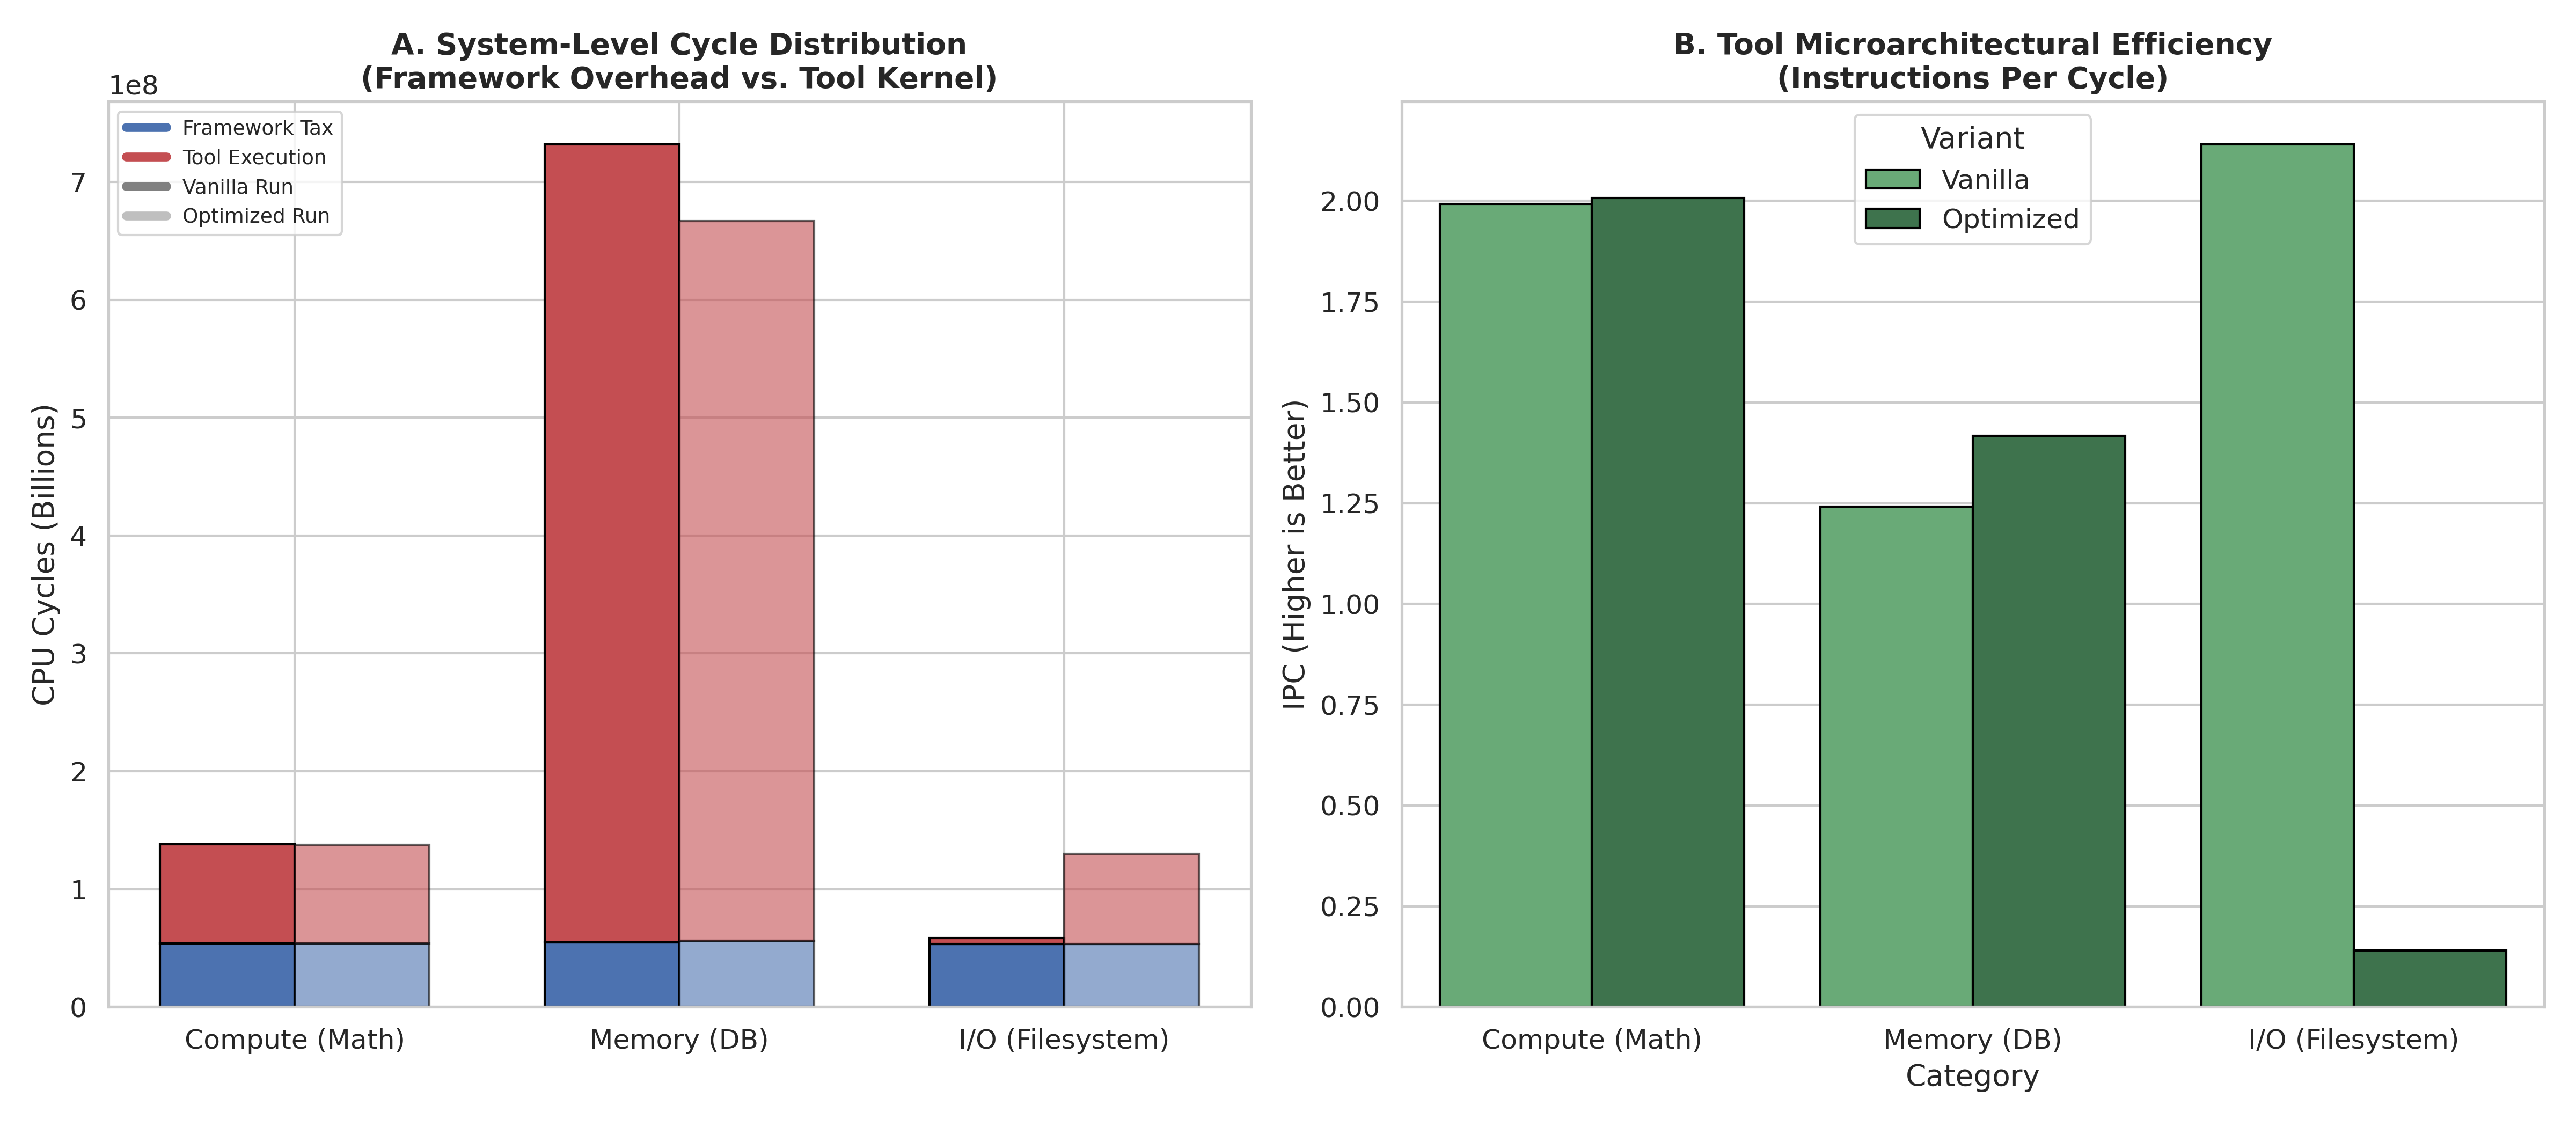
\includegraphics[width=1\textwidth]{Final_Research_Comparison.png}
    \caption{System-level cycle distribution and tool efficiency across all optimized computing domains. The contrasting panels demonstrate the ``Masking Effect'', where substantial kernel-level IPC gains (Right) fail to impact the massive framework orchestration cycles (Left).}
    \label{fig:system_masking}
\end{figure}

\section{Limitations and Discussion}
While the decoupled architecture and telemetry pipeline successfully isolated the microarchitectural overhead of agentic orchestration, several methodological constraints, concurrency limits, and hardware realities bound the generalizability of these findings.

\subsection{Methodological Constraints in Hardware Profiling}
The reliance on the Performance Application Programming Interface (PAPI) introduced a specific profiling artifact during the evaluation of highly concurrent workloads. High-level performance monitoring APIs track hardware telemetry exclusively on the calling thread. During attempts to mask I/O latency using OpenMP task parallelism in the filesystem kernel, the recorded IPC plummeted to an anomalous 0.14. 

Analysis of the execution model reveals this is a profiling blind spot rather than a true systemic degradation. The master thread, which initialized the PAPI context, entered a spin-wait state at the OpenMP synchronization barrier, executing minimal instructions while accumulating massive cycle counts. The telemetry entirely failed to capture the cumulative instruction throughput of the background worker threads. Consequently, the proposed framework accurately captures scalar execution efficiency but requires significant modification---such as thread-local PMU event sets and aggregation logic---to accurately quantify the efficiency of multi-threaded tool kernels.

\subsection{Concurrency Limits and Negative Scaling}
Beyond the profiling artifact, the application of OpenMP parallelization to the I/O-bound filesystem walk exhibited textbook negative scaling. The multithreaded kernel required 15x more CPU cycles to complete the same directory traversal as the single-threaded baseline.

Microarchitectural profiling revealed that aggregating the file count via a global atomic variable (\texttt{std::atomic}) induced severe L1 cache lock contention. The worker threads spent the majority of their execution time stalled, fighting for exclusive cache-line access to increment the shared counter. Furthermore, parallelizing disk reads for a relatively small directory hit immediate serialization bottlenecks within the OS kernel's file system drivers. This demonstrates that agentic tool frameworks cannot blindly rely on multithreading to solve I/O bottlenecks. Unless the payload size is massive, the overhead of managing thread-pools and thread synchronization costs---factors explicitly identified as CPU bottlenecks in agentic system profiling \cite{cpu_centric}---will actively degrade performance. 

\subsection{Static Workloads vs. Dynamic Real-World Variance}
To ensure deterministic execution and pristine cycle counting, generation sampling was disabled (\texttt{do\_sample=False}) and static context payloads were utilized throughout the evaluation. While necessary for rigorous microarchitectural measurement, this setup inherently masks the profound inefficiencies of real-world, dynamic agentic workloads.

In production environments, LLMs frequently hallucinate tool arguments or output malformed JSON syntax. As identified by the AI-NativeBench evaluations, this dynamic variance triggers expensive multi-turn error-correction loops, where the orchestrator must repeatedly invoke the model to correct its own formatting \cite{ai_nativebench}. This self-healing behavior exponentially increases the Agentic Tax measured in this study. 

Furthermore, static evaluation fails to capture the immense redundancy present in practical tool-calling applications. Empirical analysis of production systems demonstrates that a vast proportion of tool invocations---often exceeding 40\% in search and recommendation datasets---are redundant or highly repetitive requests \cite{toolcaching}. In dynamic, real-world deployment, the orchestration overhead is heavily influenced by the system's ability to cache and reuse these repeated calls, a factor entirely ignored by executing static, isolated payloads. Therefore, the latency penalties recorded in this pristine testing environment represent an absolute lower bound; the true systemic cost paid by production data centers is substantially higher.

\section{Conclusion and Future Work}
As the artificial intelligence industry aggressively pivots toward autonomous, multi-step agentic workflows, the underlying systems architecture must adapt to support massive tool-calling concurrency. This research introduced a deeply decoupled profiling framework to isolate and quantify the Agentic Tax---the microarchitectural overhead imposed by the LLM orchestration layer operating between the GPU generation phase and native tool execution.

The empirical evaluation yields a definitive conclusion: the current paradigm of agentic execution is crippled by an orchestration bottleneck. For lightweight tasks, the combined penalty of GPU token generation and CPU-bound string serialization can induce a 69.5x latency slowdown compared to native execution. Crucially, microarchitectural interventions proved that classical hardware optimizations at the tool level are rendered statistically irrelevant by this overarching tax. Even when deploying software prefetching to hide RAM latency and increase kernel IPC by 14.2\%, the end-to-end system speedup remained below 1\%. This Masking Effect proves that the execution bloat of the orchestration framework is so massive that it effectively swallows microarchitectural victories achieved within the tool kernels.

\subsection{Future Work: Orchestrator-Engine Co-Design}
Based on these findings, it is evident that optimizing isolated external tools provides diminishing returns. To scale agentic AI, systems engineering must pivot aggressively toward minimizing the orchestration layer and integrating decision logic directly into the serving engine. Future research and development should pursue the following critical avenues:

\textbf{1. Speculative Execution and Latency Hiding} \\
Because the standard ReAct loop is strictly serial, the LLM must halt generation and wait for the CPU to execute the tool, introducing severe latency bottlenecks \cite{paste}. To break this dependency, systems must embrace speculative execution. Frameworks like Pattern-Aware Speculative Tool Execution (PASTE) demonstrate that while agent requests are semantically diverse, their application-level control flows and data dependencies are highly predictable \cite{paste}. By decoupling control flow from data flow into a ``Pattern Tuple,'' the orchestrator can speculatively dispatch predictive tool invocations before the LLM has definitively requested them. By acting while thinking, speculative execution can overlap the CPU-bound tool latency with the GPU-bound LLM prefill phase, reducing average task completion times significantly \cite{paste}. 

Similarly, the Sutradhara architecture introduces an intelligent co-design between the orchestrator and the inference engine. By utilizing a streaming JSON parser natively within the decoding phase, the engine identifies tool call objects instantly and dispatches tools incrementally rather than waiting for the entire decode sequence to finish, shaving vital milliseconds off the FTR latency \cite{sutradhara, data_systems}. Furthermore, utilizing tool-aware prompt splitting allows the engine to begin the prefill phase for the next reasoning iteration using tool-independent context while the current tools are still executing on the CPU \cite{sutradhara}.

\textbf{2. Data-Centric Semantic Caching} \\
As agentic loops accumulate context, Key-Value (KV) cache hit rates collapse \cite{sutradhara}. Treating this redundancy purely as a generation problem is inefficient; it must be approached from a database systems perspective. By applying classical query optimization principles and capturing prompt dependencies within a templated radix tree, systems can enact proactive caching strategies to maximize KV cache reuse across batched workflows \cite{data_systems}.

However, caching the output of the external tools themselves requires handling dynamic workloads and strict Time-To-Live (TTL) freshness requirements \cite{toolcaching}. The ToolCaching framework addresses this by integrating semantic understanding with system-level signals. Utilizing the Value-Aware Adaptive Caching (VAAC) algorithm, the system evaluates request cacheability based on frequency, recency, execution cost, and network latency \cite{toolcaching}. When memory pressure occurs, VAAC preferentially retains the results of highly expensive API fetches while evicting cheap, rapid calls, reducing end-to-end tool latency by up to 34\% \cite{toolcaching}.

\textbf{3. Just-In-Time Routing and CPU-Aware Scheduling} \\
Assigning a single, static model to process an entire complex Directed Acyclic Graph (DAG) leads to massive inefficiencies, as different workflow stages demand varying cognitive capabilities \cite{ai_nativebench}. Furthermore, static assignment ignores the rapidly fluctuating system loads across the GPU cluster. Frameworks like Aragog resolve this by implementing Just-in-Time, stage-wise configuration adaptation \cite{aragog}. Aragog performs a one-time accuracy analysis when a request arrives to prune the search space into mathematically validated configurations \cite{aragog}. As the request transitions between agents, a runtime scheduler uses beam search to dynamically re-route the workload to the most available, efficient model cluster, increasing maximum serving throughput by up to 217\% \cite{aragog}. 

Complementing this routing strategy is the necessity for CPU and GPU-Aware Micro-batching (CGAM). To mitigate the specific CPU bottlenecks profiled in this analysis---such as core over-subscription and synchronization overhead---Mixed Agentic Workload Scheduling (MAWS) can intelligently balance homogeneous and heterogeneous agentic tasks, preventing the CPU orchestrator from starving the GPU engines and achieving massive latency speedups \cite{cpu_centric}.

\textbf{4. Compiled Orchestrators and Standardized Binary Protocols} \\
Finally, the industry must transition away from string-based JSON formats. Standard recursive descent JSON parsing remains a fundamental, un-vectorizable bottleneck on the CPU \cite{simdjson}. Replacing standard libraries with SIMD-accelerated parsers like \texttt{simdjson}---which utilize carry-less multiplication and branchless character classification---can drastically reduce the CPU cycles wasted on serialization \cite{simdjson}. Ultimately, future research should explore fine-tuning LLMs to output structured, in-memory binary protocols (such as Apache Arrow) natively, allowing tools to execute directly on the generation buffer without the need for intermediate CPU string serialization. 

Until the orchestration layer is treated as a high-performance networking data plane, the theoretical potential of hardware-accelerated agentic tools will remain hidden beneath the overarching execution tax.

\clearpage

% --- Bibliography mapped directly to provided ArXiv links ---
\begin{thebibliography}{99}

\bibitem{data_systems}
Efficient LLM Serving for Agentic Workflows: A Data Systems Perspective. 
\url{https://arxiv.org/abs/2603.16104v1}

\bibitem{sutradhara}
Sutradhara: An Intelligent Orchestrator-Engine Co-design for Tool-based Agentic Inference. 
\url{https://arxiv.org/abs/2601.12967}

\bibitem{cpu_centric}
A CPU-Centric Perspective on Agentic AI. 
\url{https://arxiv.org/abs/2511.00739}

\bibitem{simdjson}
Parsing Gigabytes of JSON per Second. 
\url{https://arxiv.org/abs/1902.08318}

\bibitem{paste}
Act While Thinking: Accelerating LLM Agents via Pattern-Aware Speculative Tool Execution. 
\url{https://arxiv.org/abs/2603.18897v1}

\bibitem{coupled_architectures}
Characterizing and Optimizing LLM Inference Workloads on CPU-GPU Coupled Architectures. 
\url{https://arxiv.org/abs/2504.11750v1}

\bibitem{ai_nativebench}
AI-NativeBench: An Open-Source White-Box Agentic Benchmark Suite for AI-Native Systems. 
\url{https://arxiv.org/abs/2601.09393v1}

\bibitem{toolcaching}
ToolCaching: Towards Efficient Caching for LLM Tool-calling. 
\url{https://arxiv.org/abs/2601.15335}

\bibitem{aragog}
Aragog: Just-in-Time Model Routing for Scalable Serving of Agentic Workflows. 
\url{https://arxiv.org/abs/2511.20975}

\end{thebibliography}

\clearpage

\appendix

\section{Member Contributions}
\begin{itemize}
    \item \textbf{Kunpeng Zhang:} [Specific details here]
    \item \textbf{Fazal Rehman:} [Specific details here]
    \item \textbf{TJ Grewal:} [Specific details here]
\end{itemize}

\section{Documentation and Code Instructions}
% Provide high-level instructions on how to run your code 
% (Environment setup, build commands, etc.).

\end{document}